\documentclass[12pt]{article}
\usepackage{adjustbox}
\usepackage{algorithm}
\usepackage{amsmath,amssymb}
\usepackage{tikz}
\usepackage{algpseudocode}
\usepackage[all]{xy}
\usepackage{float}
\usepackage{xcolor}

\usepackage[english]{babel}
\tikzset{every loop/.style={}}
\usetikzlibrary{arrows}
\usetikzlibrary{shapes,backgrounds}
\date{}

\title{
Hamiltonian Cycle\\}
\date{}
\author{\\Patricio T. Casurao\\Cary M. Quibada}
\newtheorem{theorem}{Theorem}

\begin{document}
\maketitle
\section{Preliminaries}
\subsection{Graphs}
\begin{itemize}
 \item \textbf{graph or general graph} - ordered triple $G=(V,E,\phi)$ where, $V\neq\varnothing$, $V \cap E = \varnothing$ and $\phi:E \rightarrow P(V)$ such that $|\phi(e)|={1,2}$ for every $e \in E$.
 \item Let G be a graph with $G = (V,E,\phi)$,
	\begin{itemize}
		\item The vertex set or $V$ is the set of vertices of G
		\item The edge set or $E$ is the set of edges
		\item $\phi(e)$ contains the endvertex/endvertices of each $e$ which are the elements of the vertex set. 
	\end{itemize}	 
\begin{figure}[h!]
\centering
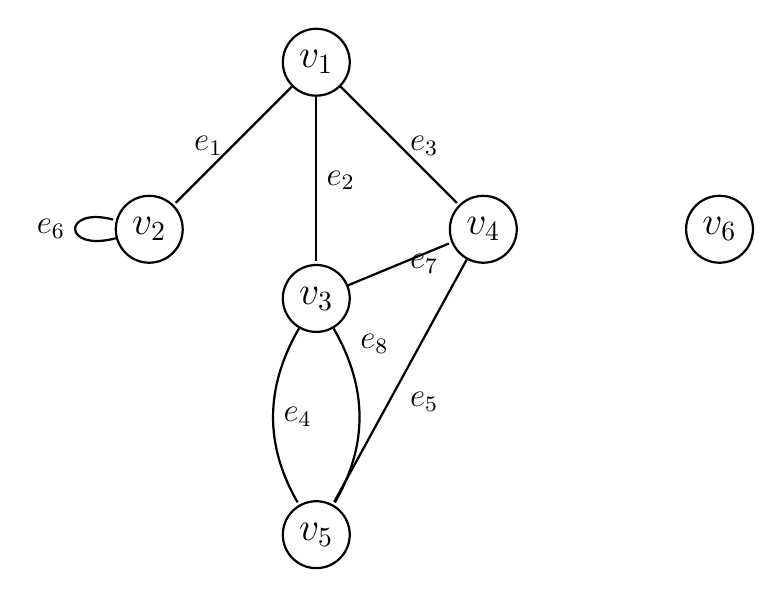
\begin{tikzpicture}[-,>=stealth',shorten >=1pt,auto,node distance=3cm,
                    thick,main node/.style={circle,draw,font=\sffamily\Large\bfseries}]

  \node[main node] (1) {$v_1$};
  \node[main node] (2) [below left of=1] {$v_2$};
  \node[main node] (3) [below of=1] {$v_3$};
  \node[main node] (4) [below right of=1] {$v_4$};
  \node[main node] (5) [below of=3] {$v_5$};
  \node[main node] (6) [right of=4] {$v_6$};
  
  \path[every node/.style={font=\sffamily\large}]
    (1) edge node [right] {$e_3$} (4)
    	edge node [left] {$e_1$} (2)
    	edge node {$e_2$} (3)
    (2) edge [loop left] node {$e_6$} (2)
    (3) edge [bend right] node  {$e_4$} (5)
        edge node [right] {$e_7$} (4)
        edge [bend left,pos=0.2] node  {$e_8$} (5)
    (4) edge node {$e_5$} (5)
	(5) 
    ;
\end{tikzpicture}
\caption{Graph G with 6 vertices and 7 edges.}
\label{graph1}
\end{figure}
In figure \ref{graph1}, 
\begin{equation}
\begin{array}{l}
G=(V,E,\phi) \\
V=\{v_1,v_2,v_3,v_4,v_5,v_6\} \\
E=\{e_1,e_2,e_3,e_4,e_5,e_6,e_7\} \\
\phi(e_1)=\{v_1,v_2\} \\
\phi(e_2)=\{v_1,v_3\} \\
\phi(e_3)=\{v_1,v_4\} \\
\phi(e_4)=\{v_3,v_5\} \\
\phi(e_5)=\{v_4,v_5\} \\
\phi(e_6)=\{v_2\} \\
\phi(e_7)=\{v_3,v_4\}
\end{array}
\end{equation}
\newpage
Let the graph $G=(V,E,\phi)$,
	\begin{itemize}
\item The vertices $u$ and $v$ are in $V$ and are \textit{adjacent/neighbor} of each other , if there is some edge $e \in E$ that has $\phi(e)=\{u,v\}$ or $\{v,u\}$. In figure 1, $v_1$ and $v_2$ are neighbors.
\item The edges $e_1$ and $e_2$ are in $E$ and are \textit{adjacent} if they contain atleast one same end vertex on their respective $\phi$, such that $\phi\{e_1\} \cap \phi\{e_2\} \neq 0$. In figure 1, $e_1$ and $e_2$ are adjacent
\item Vertex $v$ and edge $e$ are in $V$ and $E$ respectively and are \textit{incident}, if $v$ is in $\phi(e)$. In figure 1, $v_1$ and $e_3$ are incident.
\end{itemize}
Let $G=(V,E,\phi)$ be a graph with $V=\{v_1,v_2,...,v_k\}$ and $E=\{e_1,e_2,...,e_k\}$ as its vertex and edge set respectively, then,
\begin{enumerate}
	\item A \textbf{walk} in graph G is the alternating sequence of edges and vertices that start and stops with a vertex given by,
	$(v_1,e_1,v_2,e_2,...,e_k,v_k)$ such that $\phi(e_j)=\{v_{j-1},v_j\}$ for $j \in k$.
	\item A trail in G is a walk with all of its edges to be distinct.
	\item A path in G is a walk with all of its vertices to be distinct.
	\item A $u-v$ walk/trail/path is a walk starting from  the vertex $u$ and ends on the vertex $v$ with their respective characteristics.
	\item A $v-v$ walk/trail is a circuit (or closed walk/trail).
	\item A $v-v$ path is a cycle.\\
	\end{enumerate}
\item A graph $G=(V,E)$ is a \textit{cycle graph or cycle} on $n\geq3$ vertices if,
	\begin{enumerate}
		\item $V=\{v_1,v_2,...,v_n\}$
		\item $E=\{\{v_1,v_2\},\{v_2,v_3\},...,\{v_{n-1},v_{n}\},\{v_n,v_1\}\}$
	\end{enumerate}
	\begin{figure}[h!]
	\centering
	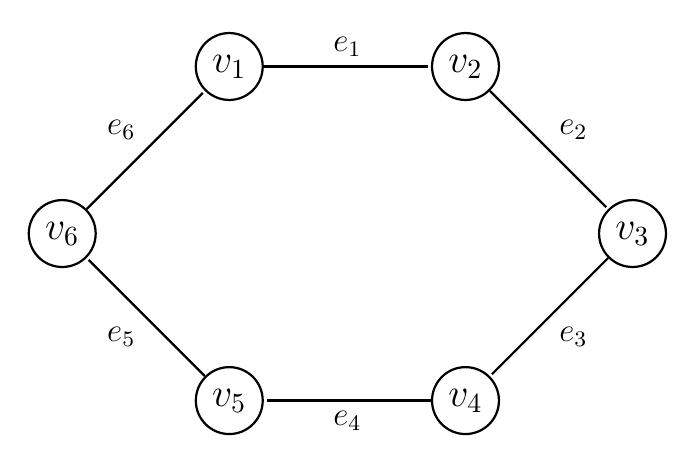
\begin{tikzpicture}[-,>=stealth',shorten >=1pt,auto,node distance=3cm,
                    thick,main node/.style={circle,draw,font=\sffamily\Large\bfseries}]

  \node[main node] (1) {$v_1$};
  \node[main node] (2) [right of=1] {$v_2$};
  \node[main node] (3) [below right of=2] {$v_3$};
  \node[main node] (4) [below left of=3] {$v_4$};
  \node[main node] (5) [left of=4] {$v_5$};
  \node[main node] (6) [above left of=5] {$v_6$};
  
  \path[every node/.style={font=\sffamily\large}]
    (1) edge node {$e_1$} (2)
    (2) edge node {$e_2$} (3)
    (3) edge node {$e_3$} (4)  
    (4) edge node {$e_4$} (5)
    (5) edge node {$e_5$} (6)
    (6) edge node {$e_6$} (1)
    ;
\end{tikzpicture}
	
	\caption{An example of a cycle graph on 6 vertices}
	\end{figure}
	\newpage
	\section{Hamiltonian Cycle Problem}
	
	A Hamiltonian cycle(/circuit) exists in a graph if there is a cycle in a graph that visits each node exactly once. If there exists a Hamiltonian circuit in a graph we can obtain a cycle graph using all the vertices in the input graph.
	\begin{figure}
	\centering
	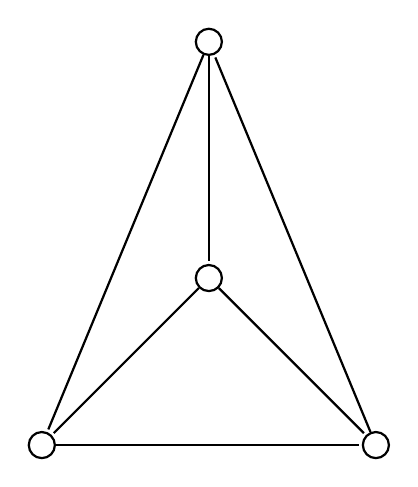
\begin{tikzpicture}[-,>=stealth',shorten >=1pt,auto,node distance=3cm,
                    thick,main node/.style={circle,draw,font=\sffamily\Large\bfseries}]

  \node[main node] (1) {};
  \node[main node] (2) [below of=1] {};
  \node[main node] (3) [below left of=2] {};
  \node[main node] (4) [below right of=2] {};
  
  \path[every node/.style={font=\sffamily\large}]
    (1) edge node {} (2)
    	edge node {} (3)
    (2) edge node {} (3)
    	edge node {} (4)
    (3) edge node {} (4)  
    (4)	edge node {} (1)
    ;
\end{tikzpicture}


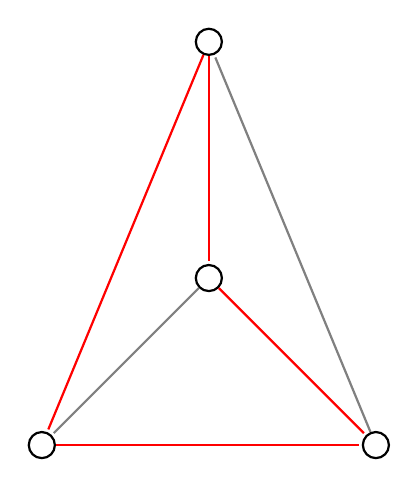
\begin{tikzpicture}[-,>=stealth',shorten >=1pt,auto,node distance=3cm,
                    thick,main node/.style={circle,draw,font=\sffamily\Large\bfseries}]

  \node[main node] (1) {};
  \node[main node] (2) [below of=1] {};
  \node[main node] (3) [below left of=2] {};
  \node[main node] (4) [below right of=2] {};
  
  \path[every node/.style={font=\sffamily\large}]
    (1) edge [color=red] node {} (2)
    	edge [color=red] node {} (3)
    (2) edge [color=gray] node {} (3)
    	edge [color=red] node {} (4)
    (3) edge [color=red] node {} (4)  
    (4)	edge [color=gray] node {} (1)
    ;
\end{tikzpicture}
\caption{An example of a graph with a Hamiltonian Cycle}
\end{figure}

\subsection{NP Completeness}

To prove that the Hamiltonian cycle problem is $NP-Complete$ we have to prove that it is in $NP$ and is in $NP-Hard$.
\subsubsection{NP}
To prove that the Hamiltonian cycle is in NP we need to find an algorithm that verifies the solution in P. Let's say we get a solution for a Hamiltonian cycle, to verify it: first, you can check if the amount of vertices in the solution is equal to the number of nodes in the input graph after that, start from any node provided by the solution and go node after node checking if they are connected by an edge and if vertices are exhausted and the end is reached: the ending vertex should be the same as the starting vertex.\\

Since there are $n$ vertices to check and $n$ edges to check as well, verifying the solution takes $n$. $n$ is a polynomial, so Hamiltonian cycle is $\in NP$ 

\subsubsection{NP Hard}

To prove that the Hamiltonian cycle problem is NP-Hard, we need to reduce an existing NP-Hard problem to a  Hamiltonian cycle. We can use the vertex cover problem for our reduction.

The vertex cover problem is a known NP-Complete problem. It objective is to find a minimum set of vertices such that every edge in the edge set of the graph is incident to at least one vertex in the set.

Proof: Given a graph $G$ and an integer $k$, we construct a Graph $G'$ such that $G$ has a vertex cover of size k if and only $G'$ has a Hamiltonian cycle. We can construct a gadget for each edge in the graph.
\begin{figure}
\centering
\scalebox{0.5}{

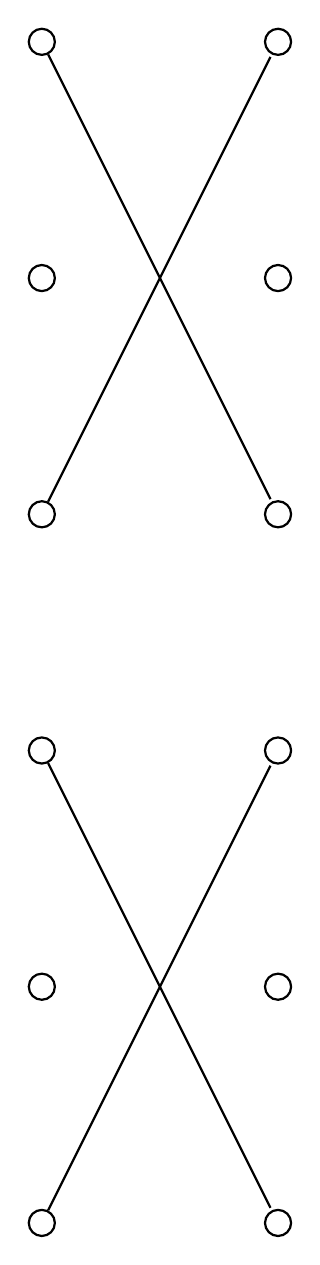
\begin{tikzpicture}[-,>=stealth',shorten >=1pt,auto,node distance=3cm,
                    thick,main node/.style={circle,draw,font=\sffamily\Large\bfseries}]

  \node[main node] (1) {};
  \node[main node] (2) [below of=1] {};
  \node[main node] (3) [below of=2] {};
  \node[main node] (4) [below of=3] {};
  \node[main node] (5) [below of=4] {};
  \node[main node] (6) [below of=5] {};
  \node[main node] (7) [right of=1] {};
  \node[main node] (8) [below of=7] {};
  \node[main node] (9) [below of=8] {};
  \node[main node] (10) [below of=9] {};
  \node[main node] (11) [below of=10] {};
  \node[main node] (12) [below of=11] {};
  
  \path[every node/.style={font=\sffamily\large}]
    (1) edge node {} (9)
    (2) 
    (3) edge node {} (7)  
    (4)	edge node {} (12)
    (5)
    (6) edge node {} (10)
    (7)
    (8)
    (9)
    (10)
    (11)
    (12)
    ;
\end{tikzpicture}
}
\caption{Gadget for representation of edge $uv$}
\end{figure}

We represent an edge as the gadget we have made. Note that we can traverse the graph in three ways such that we pass through all the vertices:

\begin{figure}
\centering
\scalebox{0.5}{

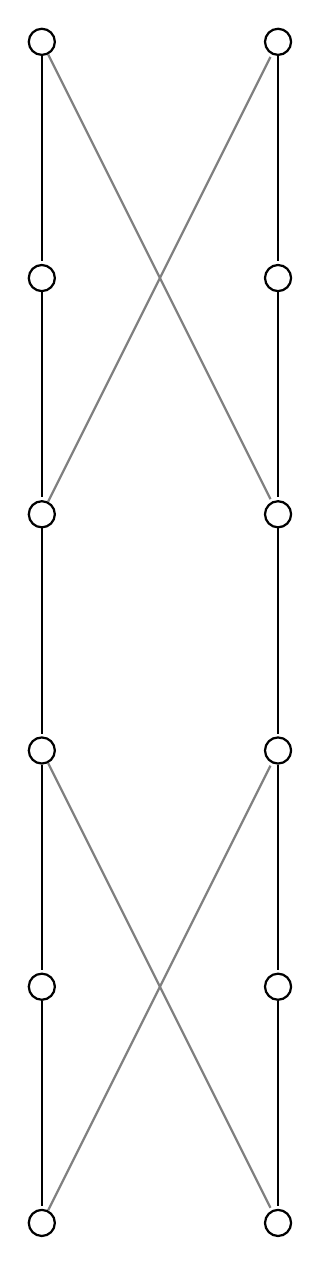
\begin{tikzpicture}[-,>=stealth',shorten >=1pt,auto,node distance=3cm,
                    thick,main node/.style={circle,draw,font=\sffamily\Large\bfseries}]

  \node[main node] (1) {};
  \node[main node] (2) [below of=1] {};
  \node[main node] (3) [below of=2] {};
  \node[main node] (4) [below of=3] {};
  \node[main node] (5) [below of=4] {};
  \node[main node] (6) [below of=5] {};
  \node[main node] (7) [right of=1] {};
  \node[main node] (8) [below of=7] {};
  \node[main node] (9) [below of=8] {};
  \node[main node] (10) [below of=9] {};
  \node[main node] (11) [below of=10] {};
  \node[main node] (12) [below of=11] {};
  
  \path[every node/.style={font=\sffamily\large}]
    (1) edge [color=gray] node {} (9)
    	edge node {} (2)
    (2) edge node {} (3)
    (3) edge [color=gray] node {} (7)  
    	edge node {} (4)
    (4)	edge [color=gray] node {} (12)
    	edge node {} (5)
    (5)	edge node {} (6)
    (6) edge [color=gray] node {} (10)
    (7) edge node {} (8)
    (8) edge node {} (9)
    (9) edge node {} (10)
    (10) edge node {} (11)
    (11) edge node {} (12)
    (12)
    ;
\end{tikzpicture}
}
\scalebox{0.5}{

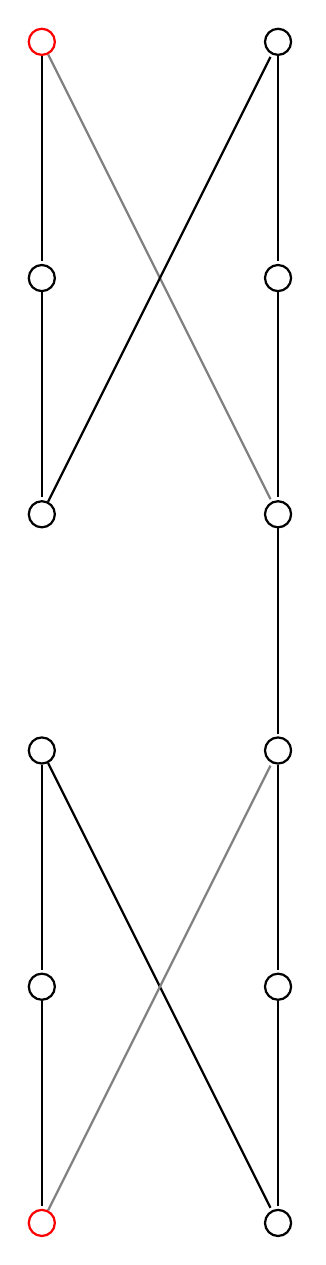
\begin{tikzpicture}[-,>=stealth',shorten >=1pt,auto,node distance=3cm,
                    thick,main node/.style={circle,draw,font=\sffamily\Large\bfseries}]

  \node[main node] (1) [color=red] {};
  \node[main node] (2) [below of=1] {};
  \node[main node] (3) [below of=2] {};
  \node[main node] (4) [below of=3] {};
  \node[main node] (5) [below of=4] {};
  \node[main node] (6) [below of=5,color=red] {};
  \node[main node] (7) [right of=1] {};
  \node[main node] (8) [below of=7] {};
  \node[main node] (9) [below of=8] {};
  \node[main node] (10) [below of=9] {};
  \node[main node] (11) [below of=10] {};
  \node[main node] (12) [below of=11] {};
  
  \path[every node/.style={font=\sffamily\large}]
    (1) edge [color=gray] node {} (9)
    	edge node {} (2)
    (2) edge node {} (3)
    (3) edge node {} (7)  
    (4)	edge  node {} (12)
    	edge node {} (5)
    (5)	edge node {} (6)
    (6) edge [color=gray] node {} (10)
    (7) edge node {} (8)
    (8) edge node {} (9)
    (9) edge node {} (10)
    (10) edge node {} (11)
    (11) edge node {} (12)
    (12)
    ;
\end{tikzpicture}
}
\scalebox{0.5}{

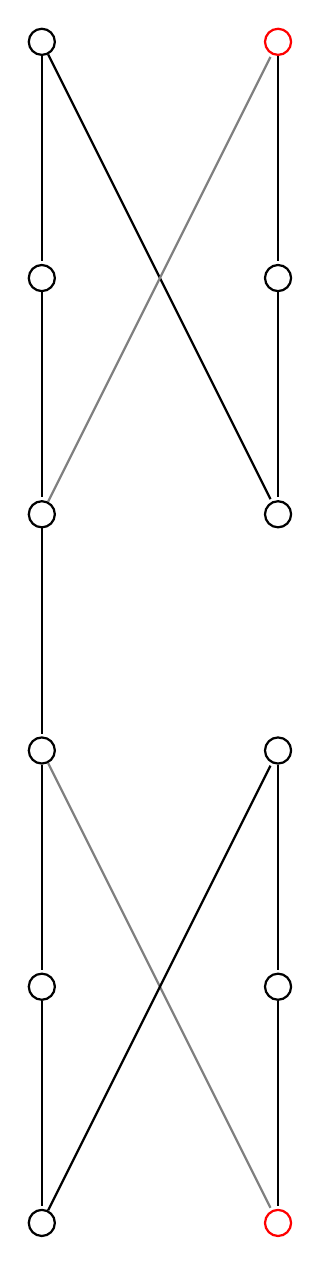
\begin{tikzpicture}[-,>=stealth',shorten >=1pt,auto,node distance=3cm,
                    thick,main node/.style={circle,draw,font=\sffamily\Large\bfseries}]

  \node[main node] (1) {};
  \node[main node] (2) [below of=1] {};
  \node[main node] (3) [below of=2] {};
  \node[main node] (4) [below of=3] {};
  \node[main node] (5) [below of=4] {};
  \node[main node] (6) [below of=5] {};
  \node[main node] (7) [right of=1,color=red] {};
  \node[main node] (8) [below of=7] {};
  \node[main node] (9) [below of=8] {};
  \node[main node] (10) [below of=9] {};
  \node[main node] (11) [below of=10] {};
  \node[main node] (12) [below of=11,color=red] {};
  
  \path[every node/.style={font=\sffamily\large}]
    (1) edge  node {} (9)
    	edge node {} (2)
    (2) edge node {} (3)
    (3) edge [color=gray] node {} (7)  
    	edge node {} (4)
    (4)	edge [color=gray] node {} (12)
    	edge node {} (5)
    (5)	edge node {} (6)
    (6) edge  node {} (10)
    (7) edge node {} (8)
    (8) edge node {} (9)
    (9) 
    (10) edge node {} (11)
    (11) edge node {} (12)
    (12)
    ;
\end{tikzpicture}
}
\caption{The left one is for traversal through $u $ and $v$ individually, middle one is for entering from $u$ passing through $v$ then exiting from $u$, the right one is the same as the middle one but with the vertices flipped.}
\end{figure}

Note that in the three cases, we enter and exit the same side. Each side of the gadget is associated with a vertex: left side of $u$ and right side of $v$. Assuming that by some order of the edges incident on a certain vertex, we can link gadgets by edges forming a chain of gadgets. In doing so for all vertices in the input $G$, we create $n$ chains with $n$ entry points and $n$ exits. Thus, we have encoded the information about $G$.

\begin{figure}
	\centering
	\includegraphics[scale=0.5]{Images/NPHardness}
\end{figure}

We set up $k$ additional vertices and connect each of these to the $n$ start points and $n$ end points of each chain.

Total size of new graph: $GE+K$ vertices and $12E+2kN+2E$ edges $\rightarrow$ construct is $P$ in size and time.

We claim this graph has a Hamiltonian cycle if and only if $G$ as a Vertex Cover of size $k$.

\begin{itemize}
	\item Suppose {$v_{1},v_2,v_3,..,v_n$} is a Hamiltonian Cycle.\\
	Assume that the cycle start at one of the $k$ vertices. It must then go through the gadgets we have presented before and we know that in the gadgets you need to pass through all the vertices in it in order to go through the end of the gadget. We also know that the gadget pertains to the vertices in the cover. To avoid visiting a vertex more than once, each chain is associated to a vertex.
	\item Now suppose we have a vertex cover of size $\leq k$.\\
	We can always add more vertices to the cover to reach $k$. For each vertex in the cover, start traversing the chain. At each entry to a gadget, check if the other vertex is in the cover and traverse the gadget accordingly.\\
	Select the selector edges to complete the circuit.
\end{itemize}
With these in mind, we have reduced vertex cover a to Hamiltonian cycle which means Hamiltonian cycle is $NP-Hard$

\section{P Algorithm}

It was stated by that finding a Hamiltonian circuit from graphs with whose vertices with degrees of 2 is in P. Which makes sense, since you just have to check the edges of each vertex if they all connect, if we end up at the start and if the iterations is equal to the number of vertices.

Conditions: input has more than 2 vertices.
All of the degrees of the vertices of the graph is degree 2. 

\begin{algorithm}
			\caption{A P Algorithm for finding a Hamiltonian Circuits}
			\begin{algorithmic}[1]
				\Require $G=(V,E)$,$Start\ vertex$ 
				\Ensure Hamiltonian Circuit
				\If{$The\ degree\ of\ all\ the\ v \in \V != 2$}
					\State No Hamiltonian Circuit
				\EndIf
				\ForAll{$v \in V$}
					\State Visit every vertex until we reach the start vertex.
				\EndFor
				\If{We have visited every vertex and we end at the start vertex}
					\State Return Hamiltonian Circuit
				\EndIf
			\end{algorithmic}
		\end{algorithm}
		
		We can observe that this algorithm is the same as checking to see if a graph is a Hamiltonian circuit. Which is a requirement in proving that the Hamiltonian Circuit problem is in NP. We can use our previous proof to say that this algorithm is in P.
\clearpage
\bibliographystyle{ieeetran}
\bibliography{references}
\end{document}